\documentclass[11pt,a4paper,titlepage]{article}
\usepackage[a4paper]{geometry}
\usepackage[utf8]{inputenc}
\usepackage[english]{babel}
\usepackage{lipsum}

\usepackage{amsmath, amssymb, amsfonts, amsthm, fouriernc, mathtools}
% mathtools for: Aboxed (put box on last equation in align envirenment)
\usepackage{microtype} %improves the spacing between words and letters

\usepackage{graphicx}
\graphicspath{ {./pics/} {./eps/}}
\usepackage{epsfig}
\usepackage{epstopdf}


%%%%%%%%%%%%%%%%%%%%%%%%%%%%%%%%%%%%%%%%%%%%%%%%%%
%% COLOR DEFINITIONS
%%%%%%%%%%%%%%%%%%%%%%%%%%%%%%%%%%%%%%%%%%%%%%%%%%
\usepackage[svgnames]{xcolor} % Enabling mixing colors and color's call by 'svgnames'
%%%%%%%%%%%%%%%%%%%%%%%%%%%%%%%%%%%%%%%%%%%%%%%%%%
\definecolor{MyColor1}{rgb}{0.2,0.4,0.6} %mix personal color
\newcommand{\textb}{\color{Black} \usefont{OT1}{lmss}{m}{n}}
\newcommand{\blue}{\color{MyColor1} \usefont{OT1}{lmss}{m}{n}}
\newcommand{\blueb}{\color{MyColor1} \usefont{OT1}{lmss}{b}{n}}
\newcommand{\red}{\color{LightCoral} \usefont{OT1}{lmss}{m}{n}}
\newcommand{\green}{\color{Turquoise} \usefont{OT1}{lmss}{m}{n}}
%%%%%%%%%%%%%%%%%%%%%%%%%%%%%%%%%%%%%%%%%%%%%%%%%%




%%%%%%%%%%%%%%%%%%%%%%%%%%%%%%%%%%%%%%%%%%%%%%%%%%
%% FONTS AND COLORS
%%%%%%%%%%%%%%%%%%%%%%%%%%%%%%%%%%%%%%%%%%%%%%%%%%
%    SECTIONS
%%%%%%%%%%%%%%%%%%%%%%%%%%%%%%%%%%%%%%%%%%%%%%%%%%
\usepackage{titlesec}
\usepackage{sectsty}
%%%%%%%%%%%%%%%%%%%%%%%%
%set section/subsections HEADINGS font and color
\sectionfont{\color{MyColor1}}  % sets colour of sections
\subsectionfont{\color{MyColor1}}  % sets colour of sections

%set section enumerator to arabic number (see footnotes markings alternatives)
\renewcommand\thesection{\arabic{section}.} %define sections numbering
\renewcommand\thesubsection{\thesection\arabic{subsection}} %subsec.num.

%define new section style
\newcommand{\mysection}{
\titleformat{\section} [runin] {\usefont{OT1}{lmss}{b}{n}\color{MyColor1}} 
{\thesection} {3pt} {} } 

%%%%%%%%%%%%%%%%%%%%%%%%%%%%%%%%%%%%%%%%%%%%%%%%%%
%       CAPTIONS
%%%%%%%%%%%%%%%%%%%%%%%%%%%%%%%%%%%%%%%%%%%%%%%%%%
\usepackage{caption}
\usepackage{subcaption}
%%%%%%%%%%%%%%%%%%%%%%%%
\captionsetup[figure]{labelfont={color=Turquoise}}

%%%%%%%%%%%%%%%%%%%%%%%%%%%%%%%%%%%%%%%%%%%%%%%%%%
%       !!!EQUATION (ARRAY) --> USING ALIGN INSTEAD
%%%%%%%%%%%%%%%%%%%%%%%%%%%%%%%%%%%%%%%%%%%%%%%%%%
%using amsmath package to redefine eq. numeration (1.1, 1.2, ...) 
%%%%%%%%%%%%%%%%%%%%%%%%
\renewcommand{\theequation}{\thesection\arabic{equation}}

%set box background to grey in align environment 
\usepackage{etoolbox}% http://ctan.org/pkg/etoolbox
\makeatletter
\patchcmd{\@Aboxed}{\boxed{#1#2}}{\colorbox{black!15}{$#1#2$}}{}{}%
\patchcmd{\@boxed}{\boxed{#1#2}}{\colorbox{black!15}{$#1#2$}}{}{}%
\makeatother
%%%%%%%%%%%%%%%%%%%%%%%%%%%%%%%%%%%%%%%%%%%%%%%%%%

\definecolor{QuestionColour}{RGB}{45, 135, 51}

\newcommand{\blankline}{\quad\pagebreak[2]}
\setlength{\parskip}{0.3em}

%%%%%%%%%%%%%%%%%%%%%%%%%%%%%%%%%%%%%%%%%%%%%%%%%%
%% DESIGN CIRCUITS
%%%%%%%%%%%%%%%%%%%%%%%%%%%%%%%%%%%%%%%%%%%%%%%%%%
\usepackage[siunitx, american, smartlabels, cute inductors, europeanvoltages]{circuitikz}
%%%%%%%%%%%%%%%%%%%%%%%%%%%%%%%%%%%%%%%%%%%%%%%%%%



\makeatletter
\let\reftagform@=\tagform@
\def\tagform@#1{\maketag@@@{(\ignorespaces\textcolor{red}{#1}\unskip\@@italiccorr)}}
\renewcommand{\eqref}[1]{\textup{\reftagform@{\ref{#1}}}}
\makeatother
\usepackage{hyperref}
\hypersetup{colorlinks=true}

%%%%%%%%%%%%%%%%%%%%%%%%%%%%%%%%%%%%%%%%%%%%%%%%%%
%% PREPARE TITLE
%%%%%%%%%%%%%%%%%%%%%%%%%%%%%%%%%%%%%%%%%%%%%%%%%%
\title{\blue INFOSYS 722 \\
Data Mining and Big Data \\
\blueb Iteration $III$}
\author{Jason Tam}
\date{\today}
%%%%%%%%%%%%%%%%%%%%%%%%%%%%%%%%%%%%%%%%%%%%%%%%%%



\begin{document}
\maketitle

\section{Business and/or Situation understanding}

The United Nations General Assembly has adopted the 2030 Agenda for Sustainable Development with 17 \href{https://www.un.org/development/desa/disabilities/envision2030.html}{\textbf{Sustainable Development Goals}} in September 2015, as shown in Figure \ref{fig:UNGoals}. These goals are established based on the principle of "leaving no one behind", which aims to include persons with disabilities in the development process, creating a sustainable world that is truly better for everyone.

\blankline

\begin{figure}[!htbp]
    \begin{center}
        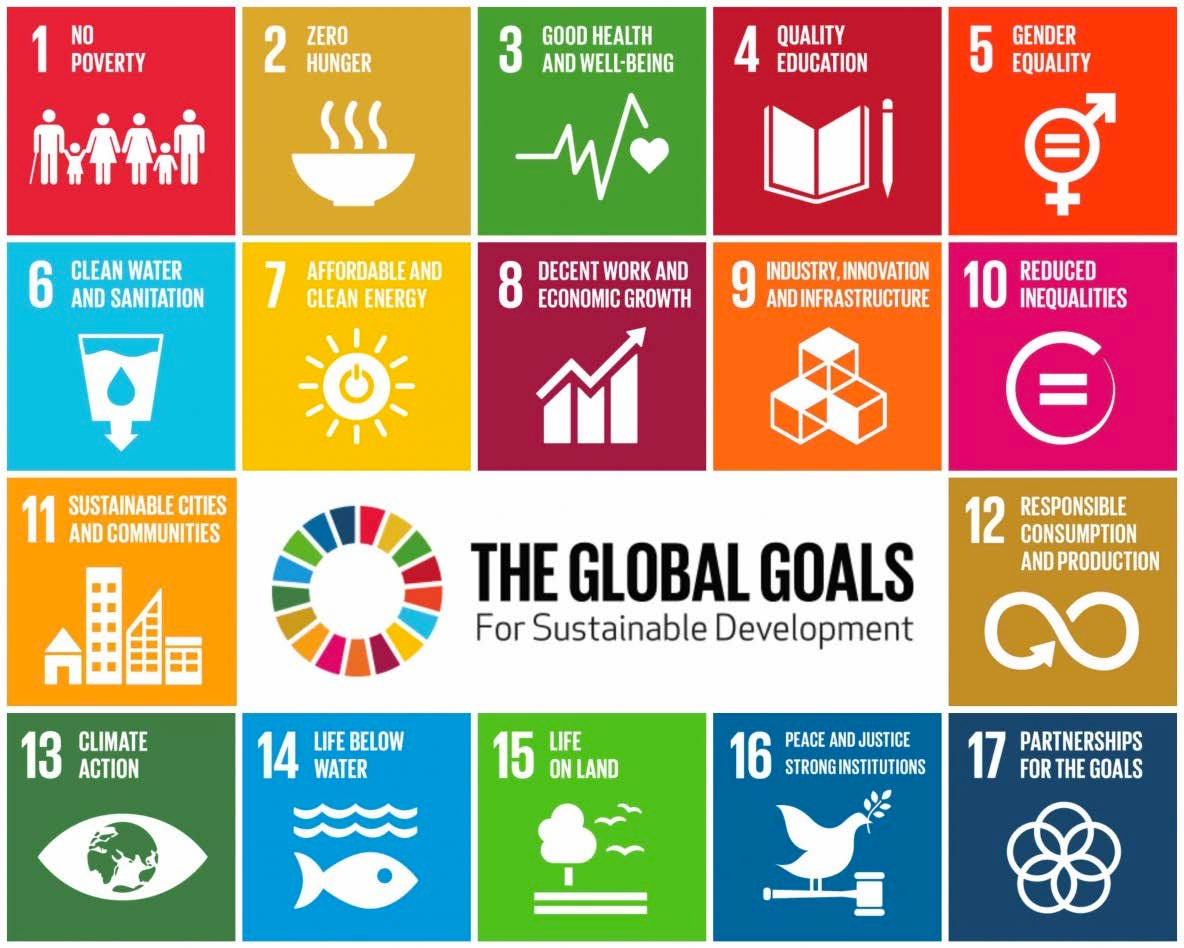
\includegraphics[width=0.8\textwidth]{UNGoals.png}
        \caption{Sustainable Development Goals from the 2030 Agenda for Sustainable Development that was adopted by the United Nations General Assembly in September 2015.}
        \label{fig:UNGoals}
    \end{center}
\end{figure}
 
While the actions to counter the effects of climate change may be categorized under the ‘Climate Action’ goal, its influence does spread to many other goals such as “Clean Water and Sanitation” and “Affordable and Clean Energy”. This makes it one of the most important issues that needs to be studied in depth to determine effective and efficient measures to counter the effects. 

\blankline

Emissions of carbon dioxide (CO2) has been identified as one of the main drivers of climate change. Modernization via industrialization has dramatically improved the quality of life in many countries in the last century, with CO2 being linked closely as a biproduct. Identifying countries with relatively low emissions while maintaining decent economy would act as a good starting point for this study, which would assist in identifying effective approaches in various aspects such as recycling and the use of environmentally sustainable energy sources that can be used as examples for other counties. This studies aims to determine if there is a general relationship between the CO$_{2}$ emmissions and the other relevant quantities including forest area percentage, total and urban population, as well as Gross Domestic Product (GDP) data of the countries listed. The obtained results may help to indicate if on optimal balance of these quantities exist to produce a thriving economy while maintaining low CO$_{2}$ emmissions.

\blankline

% \pagebreak
\section{Data understanding}

\blankline

The \href{https://www.worldbank.org/}{World Bank} contains comprehensive data sets on various macro-economic variables for a list of countries that are available for download. Historical data for some more developed countries is available further back in time compared to the others, while otherwise being reasonably comprehensive and complete. Global data of relevant variables such as population, urban population, CO2 emission, Gross Domestic Product (GDP) and forest area were obtained from the website, and each of them were available in independent comma separated (CSV) files with a common structure. \href{https://www.python.org/}{Python} and associated open source libraries such as \href{https://pandas.pydata.org/}{Pandas} are used in this instance for the analysis.

\blankline

The python codes that have been written for this analysis are stored in the \textit{Code} directory. Written functions are splitaccordingly into four different files:

\begin{itemize}
    \item \texttt{DataAnalysis.py} - Main executing code.
    \item \texttt{FitFunctions.py} - Contains functions for statistical fitting
    \item \texttt{DFFunctions.py} - Contains functions for dataframe operations
    \item \texttt{plotAnalysis.py} - Contains functions for creating plots
\end{itemize}

These CSV files are loaded into dataframe objects with the \texttt{getCSVDF} function in \texttt{FitFunctions.py}. Dataframe objects are common in analysis work with programming languages such as \href{https://www.r-project.org/}{\texttt{R}} and Python, as they are much like ordinary tables that stores structured data in the rows and columns format, with capabilities of joining to other dataframes in multiple ways that are analogous to tables in relational databases. In Python they are loaded from the Pandas library, which also contains many associated functions that are useful in manipulating the dataframes during the analysis process. 

While some of the datasets are complete up to the year 2017, others such as forest land percentage and CO$_{2}$ emissions only have complete data up to 2013. As the scope of this analysis does not require a time-dependent element, the data from the year 2013 will be used to train the models, while the 2014 set will be used to test the model.

\section{Data Preparation}

The listed countries are arranged in rows of the dataframe. Names and codes for each of them are provided as columns, as well as the name and code for the data variable. Yearly value of the variable for each year is arranged in a separate column, with the value associated to the respective country at each row. The full list of 'countries' provided in all of the CSV files are identical, which some entries are group entities with definitions that includes multiple nations. A Python dictionary was created to differentiate the standalone nations from the group entities, which is stored in the \texttt{countryTypeDict.txt} file in the same directory. It is loaded into the code through the \texttt{DFFunctions.py} class. After filtering out the group entities, there are 216 entries remaining as standalone 'countries'. Closer inspections has revealed some of the entries are inpedendent territories of a bigger nation such as \textit{Hong Kong SAR}, which explains the 216 entries of 'countries' while there are only 195 officialy recognized by the \href{http://www.un.org/en/index.html}{United Nations}.

\blankline

The 216 independent entries for this category makes it difficult to visualize data of any of the quantities for all of them simultaneously. Displaying the top 20 entries for each of the quantity has chosen to be an initial approach.

\blankline

Figure \ref{fig:LandForest2013} shows the top 20 entries for percentage of forest area. It can be observed that with the exception of Finland, Malaysia, Japan and Sweden, the rest of the entries are all small nations that commonly would not be categorized in the group of most developed nations.

\begin{figure}[!htbp]
    \begin{center}
        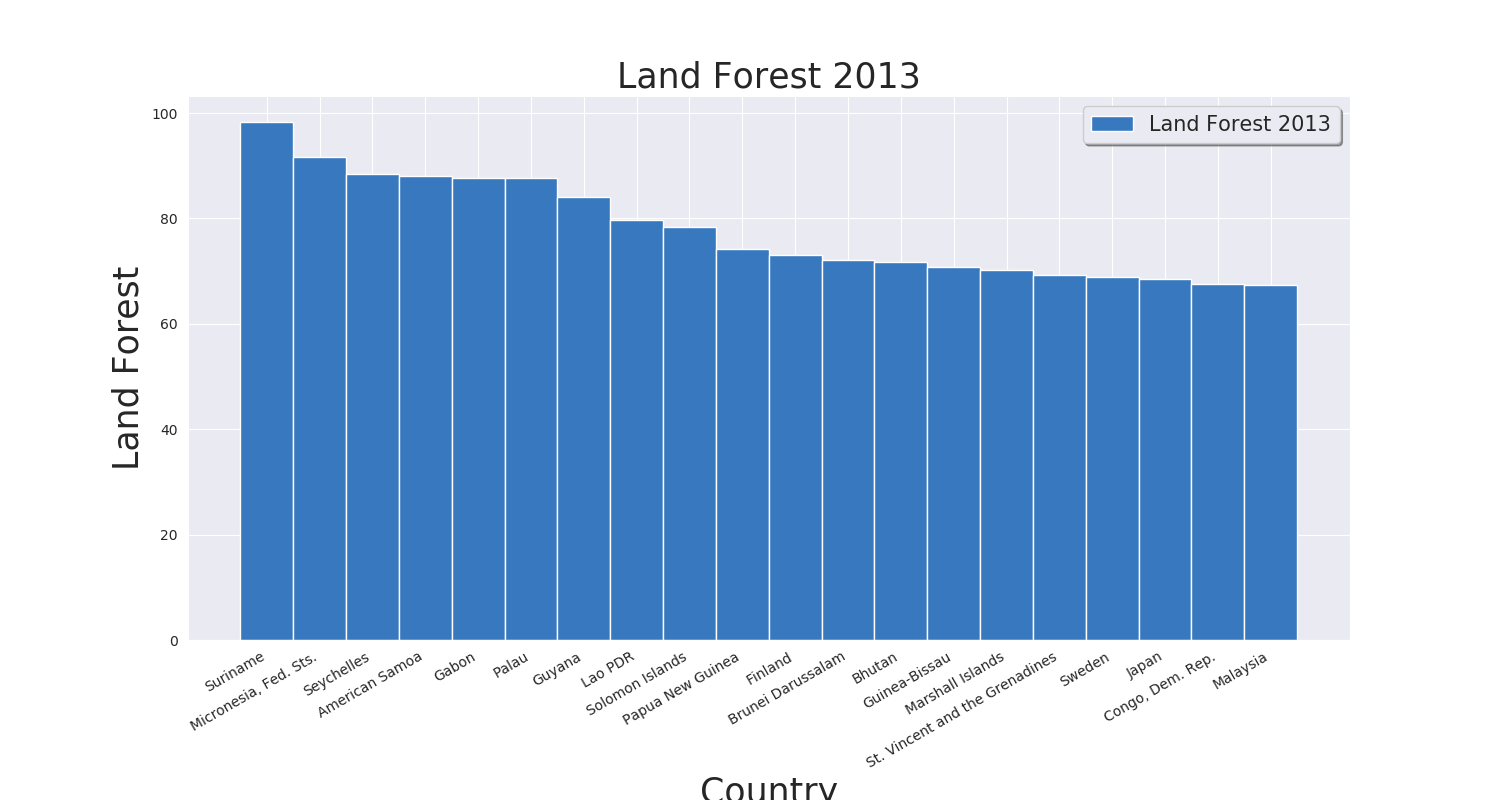
\includegraphics[width=\textwidth]{../Plots/LandForest_2013.png}
        \caption{Land Forest data of top 20 standalone nations for the year of 2013 from the \href{https://www.worldbank.org/}{World Bank}.}
        \label{fig:LandForest2013}
    \end{center}
\end{figure}

\blankline

Figures \ref{fig:CO22013} and \ref{fig:GDP2013} respectively shows the top 20 entries for CO$_{2}$ emissions and GDP data. It can be observed that there are some common entries in both lists, such as the United States, China, Germany, Russia, Brazil and South Korea. In fact with the exception of Spain and Switzerland, the rest of the top 20 nations in GDP are also in the top 20 list for CO2. With both graphs being in similar shape, it can be assumed that there is high potential that there exist a correlation between these two quantities.

\begin{figure}[!htbp]
    \begin{center}
        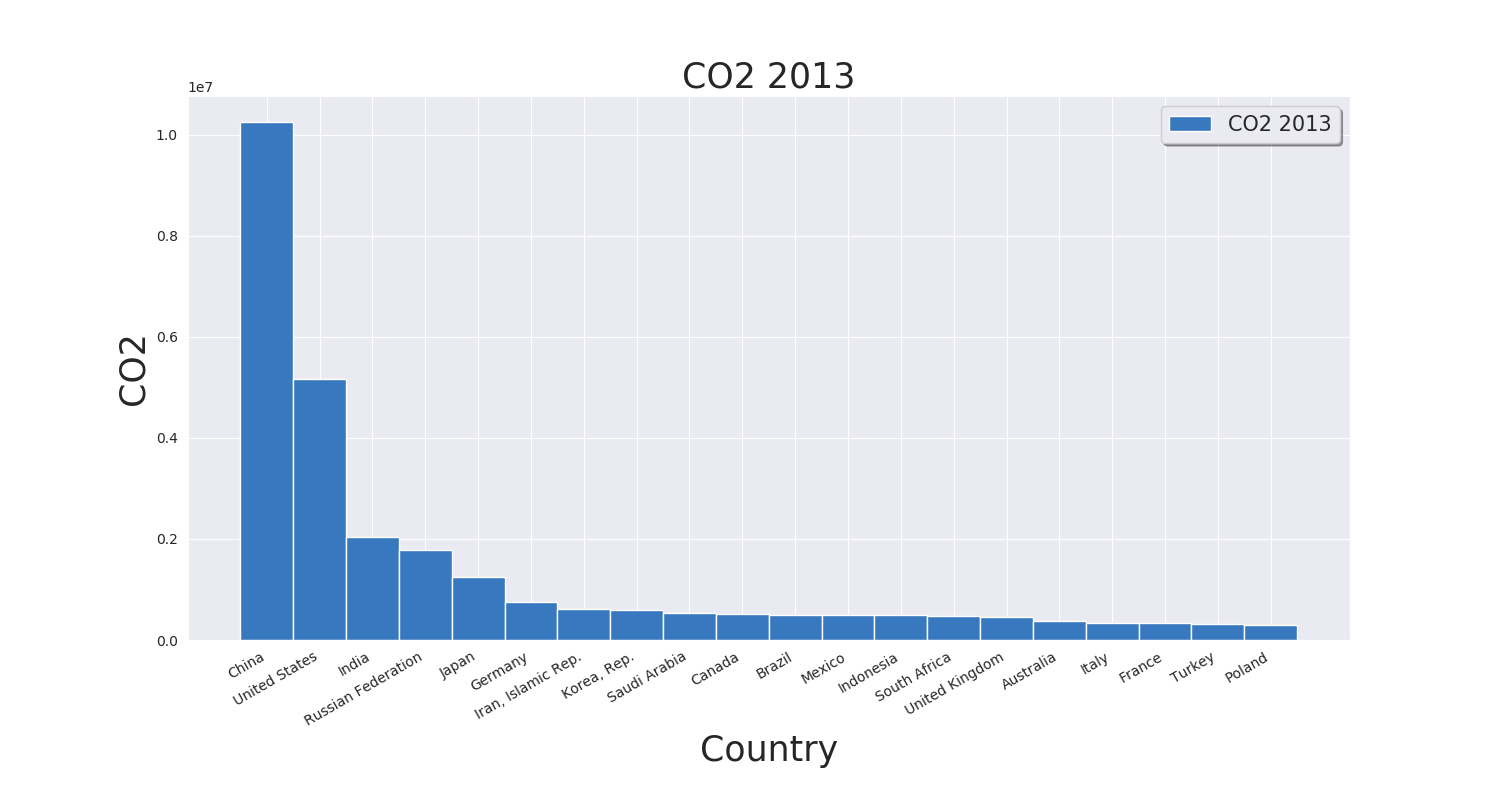
\includegraphics[width=\textwidth]{../Plots/CO2_2013.png}
        \caption{Atmospheric CO$_{2}$ data of top 20 standalone nations for the year of 2013 from the \href{https://www.worldbank.org/}{World Bank}.}
        \label{fig:CO22013}
    \end{center}
\end{figure}

\begin{figure}[!htbp]
    \begin{center}
        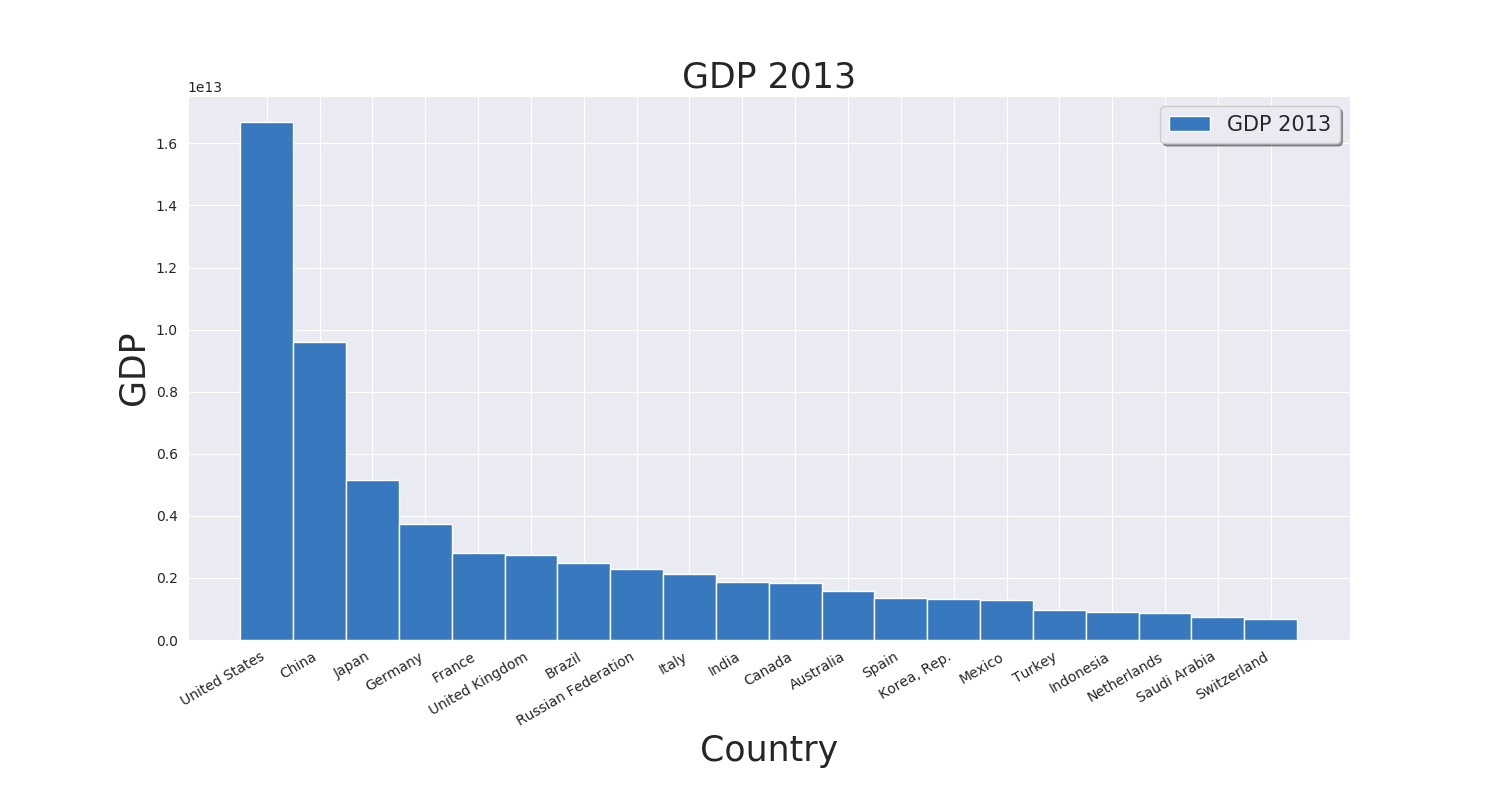
\includegraphics[width=\textwidth]{../Plots/GDP_2013.png}
        \caption{Gross Domestic Product (GDP) data of top 20 standalone nations for the year of 2013 from the \href{https://www.worldbank.org/}{World Bank}.}
        \label{fig:GDP2013}
    \end{center}
\end{figure}

The distribution of the top 20 nations with the most population shares similar shape to the previous two graphs, as shown in Figure \ref{fig:populationTotal2013}. While it can be observed the both Chain and the United States hold the top two spots in all three distributions, the other countries in this list is not as similar to the other two.

\begin{figure}[!htbp]
    \begin{center}
        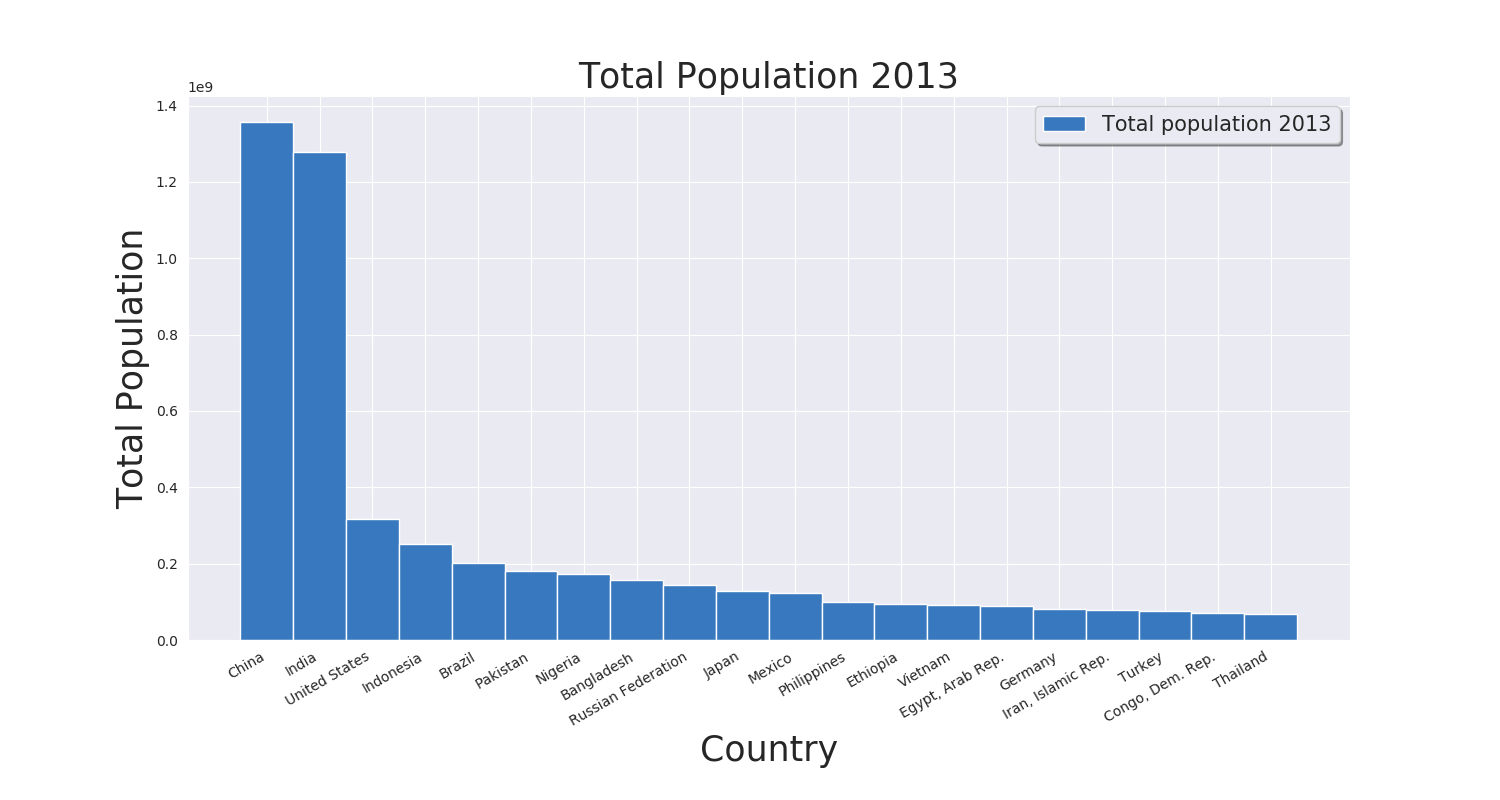
\includegraphics[width=\textwidth]{../Plots/populationTotal_2013.png}
        \caption{Total population data of top 20 standalone nations for the year of 2013 from the \href{https://www.worldbank.org/}{World Bank}.}
        \label{fig:populationTotal2013}
    \end{center}
\end{figure}

Figure \ref{fig:populationUrban2013} shows the distribution of 20 countries with the highest urban population percentage, while Figure \ref{fig:populationUrbanBottom2013} show the bottom 20. It can be observed that most of the countries that make either of these two lists are small nations, which may have little influence on the model.

\begin{figure}[!htbp]
    \begin{center}
        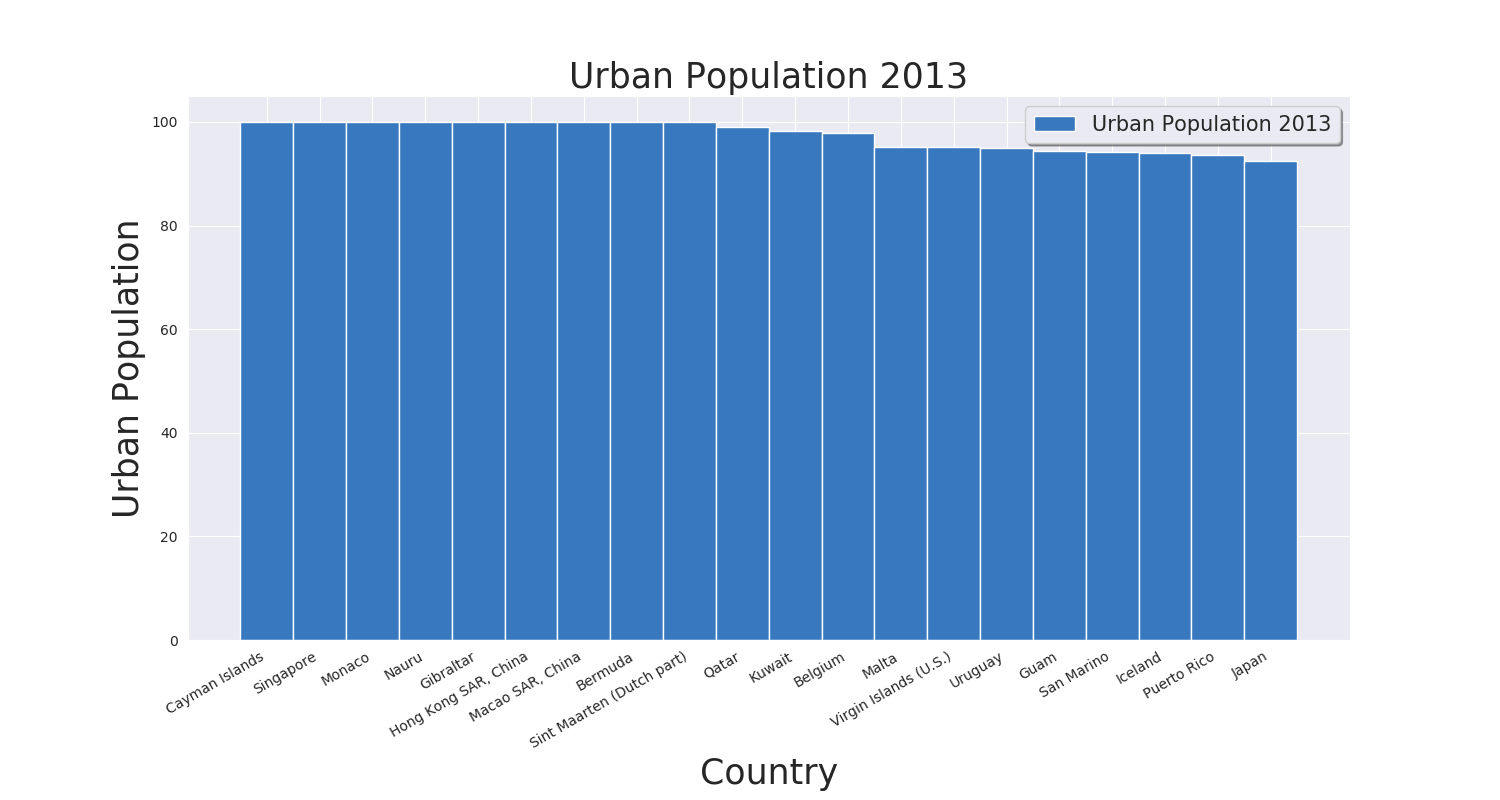
\includegraphics[width=\textwidth]{../Plots/populationUrban_2013.png}
        \caption{Urban population data of top 20 standalone nations for the year of 2013 from the \href{https://www.worldbank.org/}{World Bank}.}
        \label{fig:populationUrban2013}
    \end{center}
\end{figure}

\begin{figure}[!htbp]
    \begin{center}
        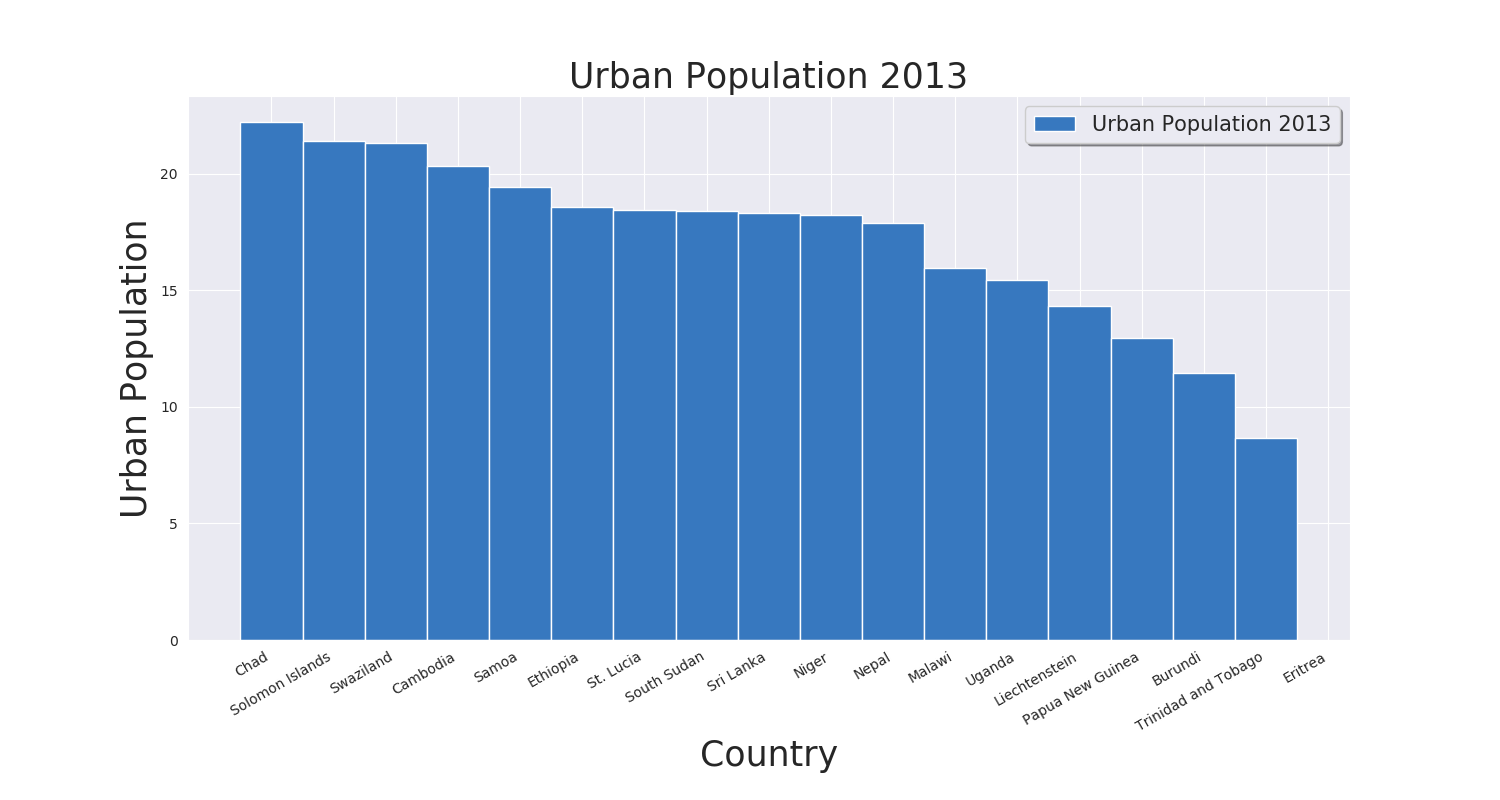
\includegraphics[width=\textwidth]{../Plots/populationUrban_2013_bottom.png}
        \caption{Urban population data of top 20 standalone nations for the year of 2013 from the \href{https://www.worldbank.org/}{World Bank}.}
        \label{fig:populationUrbanBottom2013}
    \end{center}
\end{figure}

\section{Data Transformation}

The columns with 2013 data from each of the dataframes are merged into a single one for analysis. This is performed in the main part of the analysis code (\texttt{DataAnalysis.py}):

\begin{verbatim}
dfList = [self.landForest_DF,
     self.atmosphereCO2_DF,
     self.GDP_DF,
     self.populationTotal_DF,
     self.populationUrban_DF]

trainSetupDF = pd.DataFrame({
    'Country':self.landForest_DF['Country Name'],
    'CountryType':self.landForest_DF['CountryType']
    })
testSetupDF = pd.DataFrame({
    'Country':self.landForest_DF['Country Name'],
    'CountryType':self.landForest_DF['CountryType']
    })

for i in range(0,len(dfList)):
    tempDF = dfList[i]
    # Pick year with data in every variable, particularly atmosphereCO2
    trainSetupDF[dfColumnHeaders[i]] = tempDF['2013']
    testSetupDF[dfColumnHeaders[i]] = tempDF['2014']
\end{verbatim}

\blankline

The group entities are then filtered out using the \texttt{setupAnalysisDF} function in \texttt{DFFunctions.py}. The predictors and targets for both the training data set and the testing data set are defined using the following lines in \texttt{DataAnalysis.py}:

\begin{verbatim}
train_predictors = trainDF.drop([
    'atmosphereCO2',
    'CountryType',
    'Country'], axis=1).copy()
train_target = pd.DataFrame({'atmosphereCO2':trainDF['atmosphereCO2']})

test_predictors = testDF.drop([
    'atmosphereCO2',
    'CountryType',
    'Country'], axis=1).copy()
test_target = pd.DataFrame({'atmosphereCO2':testDF['atmosphereCO2']})
\end{verbatim}

\blankline

These basic transformations of the data set can be served as input to multiple algorithms of choice for the analysis.

\section{Data-mining Algorithms and Methods Selection}

This analysis with a target quantity of CO$_{2}$ emissions and several predictors such as GDP and population data falls under the \textbf{Supervised Learning} category of the machine learning domain. Methods such as \textbf{Linear Regression} and \textbf{Random Forest} are common methods that provides a good indication on the results of a supervised learning analysis.

\section{Data Mining}

Linear regression is performed with the training data, using tools from the \texttt{statsmodel} package, with the following results:

\begin{verbatim}
                            OLS Regression Results                            
==============================================================================
Dep. Variable:          atmosphereCO2   R-squared:                       0.845
Model:                            OLS   Adj. R-squared:                  0.842
Method:                 Least Squares   F-statistic:                     254.3
Date:                Mon, 17 Sep 2018   Prob (F-statistic):           3.10e-74
Time:                        15:58:59   Log-Likelihood:                -2701.3
No. Observations:                 191   AIC:                             5413.
Df Residuals:                     186   BIC:                             5429.
Df Model:                           4                                         
Covariance Type:            nonrobust                                         
===================================================================================
                      coef    std err          t      P>|t|      [0.025      0.975]
-----------------------------------------------------------------------------------
const           -5.449e+04   7.66e+04     -0.711      0.478   -2.06e+05    9.67e+04
landForest       -248.3599   1040.340     -0.239      0.812   -2300.743    1804.023
GDP              3.016e-07      2e-08     15.084      0.000    2.62e-07    3.41e-07
populationTotal     0.0032      0.000     14.841      0.000       0.003       0.004
populationUrban    -1.7645   1096.026     -0.002      0.999   -2164.005    2160.476
==============================================================================
Omnibus:                      140.525   Durbin-Watson:                   1.931
Prob(Omnibus):                  0.000   Jarque-Bera (JB):            22618.124
Skew:                           1.659   Prob(JB):                         0.00
Kurtosis:                      56.208   Cond. No.                     4.86e+12
==============================================================================
\end{verbatim}

The results are much less than optimal, as the standard errors for the coefficients obtained are in general quite large, with the exception of GDP. Random Forest is then performed with the training data as well, utilizing the random search method to first narrow down the range of appropriate hyper-parameters, then a grid search is performed to determine them more precisely. The results are as follows:

\begin{verbatim}
Model best parameters:
{
'n_estimators': 800, 
'min_samples_split': 10, 
'min_samples_leaf': 1, 
'max_features': 'auto', 
'max_depth': 20, 
'bootstrap': False
}
Model Performance
Average Error: 56479.7575.
Accuracy = 39.85%.
Model Performance
Average Error: 75334.7533.
Accuracy = 48.96%.
Improvement of 22.87%.
\end{verbatim}

\section{Interpretation}

Figure \ref{fig:atmosphereCO2_test_residue} shows the comparison of results between the two approaches, it is a plot of residues on the test data set between the values predicted by respective models and the actual data values. The x axis displays the indicies of all of the countries to avoid confusion, and it can be observed that in general the predicted values from the trained Random Forest model is closer to the actual values compared to the linear regression approach.

\begin{figure}[!htbp]
    \begin{center}
        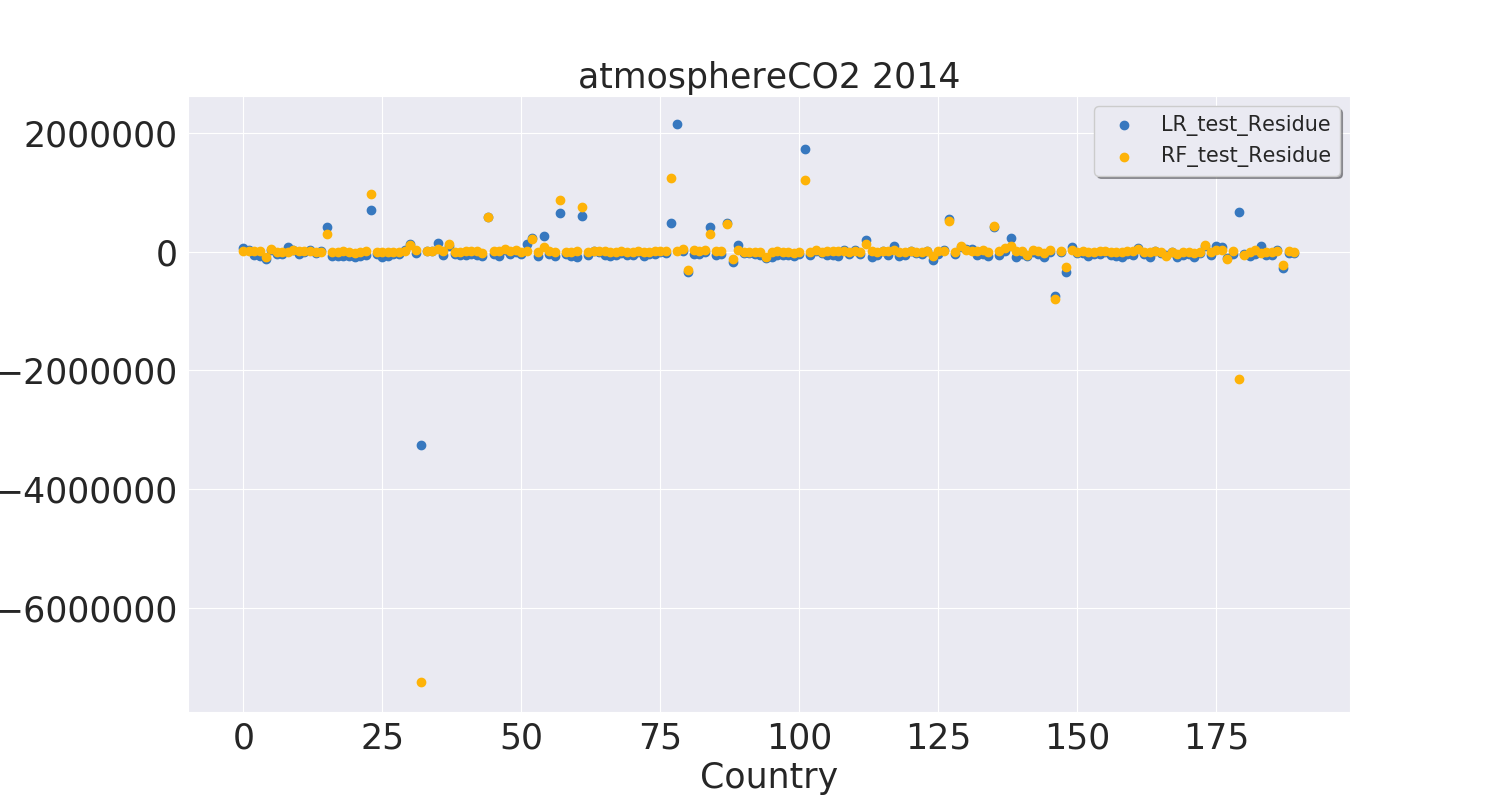
\includegraphics[width=\textwidth]{../Plots/atmosphereCO2_test_residue.png}
        \caption{Comparison between Linear Regression and Random Forest.}
        \label{fig:atmosphereCO2_test_residue}
    \end{center}
\end{figure}

Following on from this work, more models such as Neural Networks or XGBoost can be examined to determine whether a more precise prediction can be obtained, as well as attempting to drop some predictors in the linear regression approach to see if it can perform better.

\end{document}